\FloatBarrier
\chapter{Lenguaje y Tecnologías Empleadas} \label{chp:technologies}

Este capitulo aborda conceptos esenciales sobre las tecnologías usadas en el proyecto: lenguajes de programación, \textit{APIs} y herramientas de soporte. Concretamente, se trata el lenguaje \textit{C} \ref{sec:c-language}, utilizado durante todo el proyecto, las tecnologías de renderizado \ref{sec:render-technologies} y las herramientas de soporte utilizadas \ref{sec:support-technologies}.

\section{Lenguaje C} \label{sec:c-language}

\paragraph{Puntero}
Un \textbf{Puntero} es una variable que almacena una dirección en memoria de otra variable. 

Cabe mencionar que también es posible crear un puntero a una \textbf{función}:
\lstinputlisting[
    float,
    floatplacement=htp,
    language=C,
    label=cod:example-function-pointer,
    caption=Ejemplo de puntero a función en C
]{code/c_example_function_pointer.c}


\paragraph{Reserva y liberación de memoria}
En el lenguaje \textit{C}, la gestión de memoria \cite{webCppreferenceMemory} puede ser controlada por el usuario, lo que exige una gran responsabilidad por su parte. Aunque se prefiere siempre que sea posible que el sistema sea el que realice esta gestión, a veces es necesario: por ejemplo, una función que debe asignar espacio a un \textit{array} con un número de elementos no predefinido. En estos casos, puede hacerse uso de funciones como \textit{malloc} o \textit{calloc}, que inicializan memoria a petición del usuario; si se desea modificar el tamaño de esta memoria, puede utilizarse \textit{realloc} en lugar de una asignación nueva. Una vez terminadas las tareas pertinentes a la asignación de esta memoria solicitada, es necesario liberarla con \textit{free} y, para ser riguroso, darle un valor \textit{NULL} al puntero para evitar posibles confusiones respecto a la disponibilidad del mismo. 

\section{Tecnologías de renderizado} \label{sec:render-technologies}
En esta sección se describen, desde el punto de vista de la programación, las \textit{APIs} utilizadas.

Respecto a la sección \ref{sub:opengl}, que explica los conceptos pertenecientes a \textit{OpenGL} más importantes:
\begin{enumerate}

    \item En el apartado \ref{par:ogl-introduction} se presentan los conceptos necesarios de OpenGL. 
    
    \item En \ref{par:ogl-buffers} se describe cómo utilizar los \textit{buffers} con el fin de comunicarse con la \textit{GPU}.

    \item En \ref{par:ogl-shader-flow} se describe el flujo de \textit{shaders} que recorre una aplicación general que use \textit{OpenGl}.

    \item En \ref{par:ogl-uniforms} se explica el tipo de variable \textit{uniform}, utilizado para comunicarse directamente con valores de \textit{shaders}.

    \item En \ref{par:ogl-vertices-attributes} se describe cómo indicar al \textit{shader} qué valores utilizar y dónde se encuentran dentro de los \textit{buffers}, mencionados previamente.

    \item En \ref{par:ogl-shader-compilation} y \ref{par:ogl-program-creation} se describe con ejemplos de código el proceso para crear \textit{shaders} y un programa a partir de éstos.

    \item En la sección \ref{sub:glsl} se describe el lenguaje \textit{GLSL}, utilizado con el fin de programar \textit{shaders} para \textit{OpenGL}.
    
\end{enumerate}



\subsection{OpenGL} \label{sub:opengl}

Aunque también mencionado en el apartado \ref{sec:apis-render}, de las API existentes, \textit{OpenGL} y \textit{Vulkan}, en este trabajo se ha decidido usar \textit{OpenGL}, ya que es una \textit{API} muy utilizada y estable, a la par que altamente flexible (aunque no al nivel de \textit{Vulkan}).

\paragraph{Funcionamiento principal} \label{par:ogl-introduction}

Existen dos formas de utilizar \textit{OpenGl}: \textit{Immediate mode} y \textit{core-profile}. El primer modo es más fácil de entender y usar, aunque tiene funciones obsoletas y no se aconseja su uso. La manera recomendada de programar es con \textit{core-profile}, una división de la especificación con funcionalidades modernas. La especificación de \textit{OpenGL} permite extensiones para que los desarrolladores no necesiten esperar a una nueva versión.

\textit{OpenGL} se puede entender como una gran máquina de estados, llamándose a cada uno de ellos un \textbf{contexto}. Este contexto puede ser modificado por funciones y utilizado por otras. El código está escrito en \textit{C}, aunque permite derivaciones para distintos lenguajes. Se usan \textbf{objetos}: cada objeto es un conjunto de opciones que representan un \textit{subset} del estado de \textit{OpenGL}. Por ejemplo, un objeto podría representar el tamaño y colores de una ventana.

Los objetos se crean, se modifican y se utilizan mediante la \textit{API}, y la información se almacena fuera de la vista del programador. Esto permite una flexibilidad y reusabilidad increíble, pues se pueden crear varios objetos y vincularlos para dibujarlos de forma rápida.

El extracto de código \ref{cod:example-opengl-object} podría ser (son comandos ficticios) un ejemplo de creación y manipulación de un objeto:
\lstinputlisting[
    float,
    floatplacement=!htp,
    language=C,
    label=cod:example-opengl-object,
    caption=Ejemplo de objeto en OpenGL
]{code/c_example_opengl_object.c}

\paragraph{Buffers} \label{par:ogl-buffers}

A continuación se detallará la especificación de vértices \cite{webVertexSpecDocs} en \textit{OpenGL}.

\begin{itemize}
    \item El \textit{Vertex Buffer Object} (VBO) es un\textit{buffer} que puede almacenar una gran cantidad de vértices en memoria. El objetivo es envíar el mayor número de datos a la vez posible.

    \item Un \textit{Vertex Array Object} (VAO) es un \textit{buffer} enlazable, como es el \textit{VBO}. Almacena la configuración de los atributos de los vértices. Está fuertemente vinculado al \textit{VBO}, ya que el \textit{VAO} almacena la configuración de los vértices almacenados en él. El \textit{VAO} almacena las llamadas a atributos y vértices, por lo que para dibujar, una vez configurado, sería necesario simplemente vincularlo. Cabe mencionar que, si la configuración o el \textit{VBO} cambiase, sería necesario actualizar el \textit{VAO}.

    \item Un \textit{Element Buffer Object} (EBO), también llamado \textit{Index Buffer}, permite almacenar en él indices que referencian vértices en el \textit{VBO}. En vez de duplicar vértices, pueden referenciarse múltiples veces. Por ejemplo, un cuadrado contiene 2 triángulos y 6 vértices. Utilizando un \textit{EBO}, podrían declararse 4 vértices e indicar el orden en el que se utilizan para crear los triángulos.
\end{itemize}

En el ejemplo \ref{cod:example-creation-vbo-vao} se muestra un ejemplo de creación de los \textit{buffers VBO} y \textit{VAO}. Una vez creados y configurados, en la función \textit{display} ha de vincularse el \textit{VAO} para cargar los vértices y su configuración, como en el ejemplo \ref{cod:example-usage-vbo-vao}.
\lstinputlisting[
    float,
    floatplacement=!htp,
    language=C,
    label=cod:example-creation-vbo-vao,
    caption=Ejemplo de creación de los objetos VBO y VAO.
]{code/c_example_creation_vbo_vao.c}

\lstinputlisting[
    float,
    floatplacement=!htp,
    language=C,
    label=cod:example-usage-vbo-vao,
    caption=Ejemplo de uso de los objetos VBO y VAO.
]{code/c_example_usage_vbo_vao.c}

\FloatBarrier

El \textit{EBO} puede usarse para dibujar un cuadrado. Se debe añadir después de vincular el \textit{VAO}, dejando el resto de la misma manera. La función de \textit{display} es idéntica, aunque se sustituye \textit{glDrawArrays} por \textit{glDrawElements}. El ejemplo \ref{cod:example-creation-ebo} se muestra la creación de este \textit{buffer EBO} y en el ejemplo \ref{cod:example-usage-ebo} el uso de éste.

\lstinputlisting[
    float,
    floatplacement=!htp,
    language=C,
    label=cod:example-creation-ebo,
    caption=Ejemplo de creación de EBO.
]{code/c_example_creation_ebo.c}

\lstinputlisting[
    float,
    floatplacement=!htp,
    language=C,
    label=cod:example-usage-ebo,
    caption=Ejemplo de uso de EBO.
]{code/c_example_usage_ebo.c}

\FloatBarrier
\paragraph{Flujo de shaders} \label{par:ogl-shader-flow}

El flujo de shaders \cite{webOGLShaderPipe} de \textit{OpenGL} puede dividirse en 6 etapas fundamentales: \textit{Vertex Shader}, \textit{Tesselation}, \textit{Geometry Shader}, \textit{Primitive Assembly}, \textit{Rasterization}, \textit{Fragment Shader} y \textit{Tests and Blending}. Hay algunas fases en las que el programador puede introducir su propia implementación, como se mostrará más adelante.

Se usa un lenguaje especial de \textit{OpenGL} para \textit{shaders}, llamado \textit{GLSL}, para compilar y generar estos \textit{shaders}. Este lenguaje se tratará más adelante.

\begin{enumerate}
    \item \textbf{Vertex Shader}. Se transforman vectores de posición de los vértices en otros diferentes, generalmente 3D.
    
    \item \textbf{Tessellation}. Se subdivide la geometría compleja en Primitivos más simples.
    
    \item \textbf{Geometry Shader}. Se modifican, añaden o eliminan formas. Por ejemplo, romper un triángulo en tres, eliminar formas que no necesita o cambiar un punto en un cuadrado.
    
    \item \textbf{Primitive Assembly}. Se toman los vértices procesados y se agrupan en formas simples, como puntos, líneas o triángulos.
    
    \item \textbf{Rasterization}. Se transforman formas 3D en piezas 2D llamadas fragmentos (potenciales píxeles). En esta fase se determina qué píxeles en la pantalla cubre cada forma y qué datos lleva cada fragmento.
    
    \item \textbf{Fragment Shader}. En este paso se decide cómo se verá cada fragmento, es decir, color, luces, sombras, textura, etc.
    
    \item \textbf{Tests and Blending} (Per-Sample Operations). En este paso final se decide qué fragmentos finalmente ocuparán píxeles en la pantalla. Se hacen pruebas como el \textit{Depth Test}, el \textit{Stencil Test} o el \textit{Scissor Test}. Después de estas pruebas se crea la imagen final con los fragmentos restantes.

\end{enumerate}

\begin{figure}[htp]
    \centering
    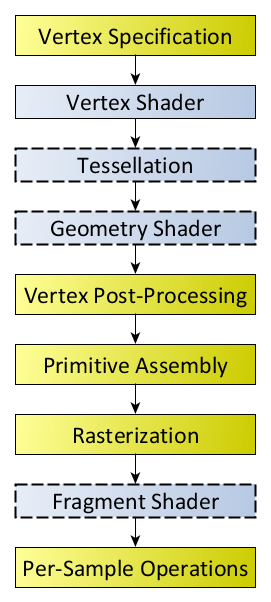
\includegraphics[height=0.8\textheight]{figures/diagrams/RenderingPipeline.png}
    \caption{Diagrama de Khronos que describe el flujo de shaders en OpenGL.}
    \label{fig:shader-pipeline}
\end{figure}

\FloatBarrier
\paragraph{Uniforms} \label{par:ogl-uniforms}

Los \textit{uniforms} son una manera de enviar datos de la aplicación en \textit{CPU} a los \textit{shaders} en \textit{GPU}. Son variables globales y pueden ser accedidas por cualquier \textit{shader}. Se añade la palabra clave \textit{uniform} a la variable en el \textit{shader} para convertirla en \textit{uniform}. Esta variable debe ser declarada en el \textit{shader}, de la misma forma que cualquier variable en \textit{GLSL}, aunque con el prefijo \textit{uniform}. Para acceder a ella desde el código \textit{C}, primero se debe localizar el atributo y entonces, dar un valor a la variable. En la figura \ref{cod:example-uniform} se muestra un ejemplo.

\lstinputlisting[
    float,
    floatplacement=!htp,
    language=C,
    label=cod:example-uniform,
    caption=Ejemplo de uso de variables Uniform.
]{code/c_example_uniform.c}

\FloatBarrier
\paragraph{Atributos de vértices} \label{par:ogl-vertices-attributes}

Para indicarle a \textit{OpenGL} cómo utilizar los datos que ha recibido, es necesario indicarlo explícitamente. Por ejemplo, si los vértices tienen 3 coordenadas, siendo cada una de ellas float, que usualmente son 4 bytes, esto significa que cada vértice serán 12 bytes, y si el polígono deseado fuera un triángulo, serían 3 vértices: 36 bytes. Se debe tener en cuenta que no hay espacio entre los valores en este caso. Un ejemplo de configuración de atributos sería la figura \ref{cod:example-attributes}.

\lstinputlisting[
    float,
    floatplacement=!htp,
    language=C,
    label=cod:example-attributes,
    caption=Ejemplo de configuración de atributos.
]{code/c_example_attributes.c}

Los argumentos de \textit{glVertexAttribPointer} son:
\begin{enumerate}
    \item \textbf{Índice}. Posición del atributo. Puede definirse en el shader o conseguirse dinámicamente.

    \item \textbf{Tamaño} del atributo. 

    \item \textbf{Tipo} de dato. Las coordenadas se guardan como \textit{float}.

    \item \textbf{Normalización}. En este caso, las coordenadas están ya normalizadas previamente, por lo que se deja en falso.

    \item \textbf{Stride}. Es el espacio entre atributos consecutivos. Si es \textit{0}, se asumirá que los datos siguen uno detrás del otro sin espacio entre ellos.

    \item \textbf{Offset}. Es donde empieza la posición de los datos en el \textit{buffer}. Requiere un puntero a \textit{void}.

\end{enumerate}

\FloatBarrier
\paragraph{Compilación de un shader} \label{par:ogl-shader-compilation}

Con el propósito de mantener la sencillez en el ejemplo, el código \textit{GLSL} se almacenará en constantes dentro del código \textit{C}, el cual se le proporciona a \textit{OpenGL} y se compila; en el ejemplo \ref{cod:example-shader-compilation} se muestra este concepto.

\lstinputlisting[
    float,
    floatplacement=!htp,
    language=C,
    label=cod:example-shader-compilation,
    caption=Ejemplo de compilación de un shader
]{code/c_example_shader_compilation.c}

\FloatBarrier
\paragraph{Creación de un programa} \label{par:ogl-program-creation}

Una vez se tienen los \textit{shaders} compilados por separado, es necesario enlazarlos para combinarlos. Esto se hace mediante un \textbf{programa}. Se vinculan los shaders a este programa, que se activa cuando se renderizan objetos. Las salidas de cada \textit{shader}, entonces, se vinculan a las entradas del siguiente. El código necesario para la creación del programa podría ser como el de la figura \ref{cod:example-shader-program}.

\lstinputlisting[
    float,
    floatplacement=!htp,
    language=C,
    label=cod:example-shader-program,
    caption=Ejemplo de creación de un programa
]{code/c_example_shader_program.c}

\subsection{GLSL} \label{sub:glsl}

Los shaders deben ser compilados en tiempo de ejecución. Aunque no  se haya profundizado en el lenguaje \textit{GLSL} \cite{webGLSLDocs}, es sencillo de entender una vez aprendido \textit{C}.

El código de la figura \ref{cod:example-vertex-shader} es un ejemplo muy básico de un \textit{Vertex Shader} que simplemente pasa las coordenadas al \textit{shader}, sin manipularlas:
\lstinputlisting[
    float,
    floatplacement=!htp,
    language=GLSL,
    label=cod:example-vertex-shader,
    caption=Ejemplo de Vertex Shader
]{code/glsl_example_vertex_shader.vert}

La primera línea indica la versión que se utiliza, que es semejante a la versión de \textit{OpenGL} que se esté usando (3.3). La segunda línea indica la posición en la que se encuentra el dato \textit{aPos}, que es un vector de 3 dimensiones. Este sería el vector que indica la posición de un vértice. La posición se transporta a un vector de 4 dimensiones, en la que la última coordenada es un dato llamado \textit{perspective division}, en la función principal del \textit{shader}.

\FloatBarrier

El código de la figura \ref{cod:example-fragment-shader} es un ejemplo muy básico de un \textit{Fragment Shader} que hace que todos los colores sean el naranja.

\lstinputlisting[
    float,
    floatplacement=!htp,
    language=GLSL,
    label=cod:example-fragment-shader,
    caption=Ejemplo de Fragment Shader
]{code/glsl_example_fragment_shader.frag}

La instrucción out hace que devuelva una variable: \textit{FragColor}, que decide el color final. En este caso, es un vector de 4 dimensiones, que indica los tres colores primarios: rojo, verde y azul (RGB) y el valor alpha (opacidad).

\FloatBarrier
\section{Herramientas de soporte} \label{sec:support-technologies}

En esta sección se tratarán herramientas de soporte, útiles para la gestión y organización del proyecto, tanto en la estructura como en el código, tales como \textit{CMake} \ref{sub:support-cmake}, que gestiona la compilación y dependencias, \textit{GLEW} \ref{sub:support-glew}, que elimina la necesidad de obtener las funciones de \textit{OpenGL} manualmente, \textit{Freeglut} \ref{sub:support-freeglut}, que gestiona la creación de ventanas, o \textit{Git} \ref{sub:support-git}, que gestiona el control de versiones.

\subsection{CMake} \label{sub:support-cmake}
Se usará \textit{CMake} \cite{webCMakeDocs} para gestionar dependencias y compilación del proyecto.

\textit{CMake} maneja dependencias de forma estable y es beneficioso a largo plazo, cuando el código empieza a aumentar de tamaño y comienza a ser insostenible compilar a mano. Otra alternativa sería manualmente escribir \textit{Makefile}. Se consideró más útil y profesional usar \textit{CMake}, ya que tiene un nivel de abstracción sobre los \textit{Makefile} muy pulido y efectivo que costaría replicar a mano.

\FloatBarrier
\subsection{GLEW} \label{sub:support-glew}
Las funciones de \textit{OpenGL} se cargan de maneras diferentes según la plataforma en la que nos encontremos. En \textit{GNU/Linux}, bajo la implementación de \textit{Mesa} \cite{webMesaDocs}, están dinámicamente enlazadas, por lo que hay que recuperarlas de memoria. En otras plataformas es distinto, por lo que \textit{GLEW} es muy útil para resolver este problema.

\textit{GLEW} \cite{webGLEW} inicializa las funciones de \textit{OpenGL} de forma agnóstica al sistema operativo. Esto libera al programador de una tediosa carga, pues hacerlo de forma manual sería fatigador y la mejora en rendimiento sería mínima o nula. El código necesario para la inicialización de \textit{GLEW} es sencillo y se muestra en la figura \ref{cod:example-glew}.

\lstinputlisting[
    float,
    floatplacement=!htp,
    language=C,
    label=cod:example-glew,
    caption=Ejemplo de inicialización de GLEW
]{code/c_example_glew.c}

\FloatBarrier
\subsection{Freeglut} \label{sub:support-freeglut}
\textit{Freeglut} \cite{webFreeglut} nace como alternativa a \textit{GLUT} \cite{specsGLUT}, una biblioteca ya abandonada. Se encarga de todas las tareas específicas al sistema operativo necesarias para crear ventanas, inicializar contextos de \textit{OpenGL}, gestionar eventos de entrada y permite crear programas realmente portables con \textit{OpenGL}. El codigo necesario para inicializar \textit{Freeglut} podría ser como en la figura \ref{cod:example-glut}:

\lstinputlisting[
    float,
    floatplacement=!htp,
    language=C,
    label=cod:example-glut,
    caption=Ejemplo de inicialización de Freeglut
]{code/c_example_glut.c}

\FloatBarrier

\subsection{Git} \label{sub:support-git}

La tecnología \textit{Git} se ha utilizado durante todo el proyecto como software de \textbf{control de versiones}, haciendo gran uso de las ramas para distintas funcionalidades, las cuales evitan un posible colapso irremediable permitiendo deshacer cambios rápidamente.
